
\title{Multicore MIL}

\author{}

\maketitle

\section{Introduction}
%
We adapt MIL to a multicore setting. MIL programs become threads, but are otherwise to a large extent unchanged from \cite{mil}. Multicopy atomicity: IRIW - if thread 1 sees write by thread 2 then thread 3 sees it as well. Same memory model as in flat \cite{mca-flat}.
%%
\begin{figure}[t]
\begin{center}
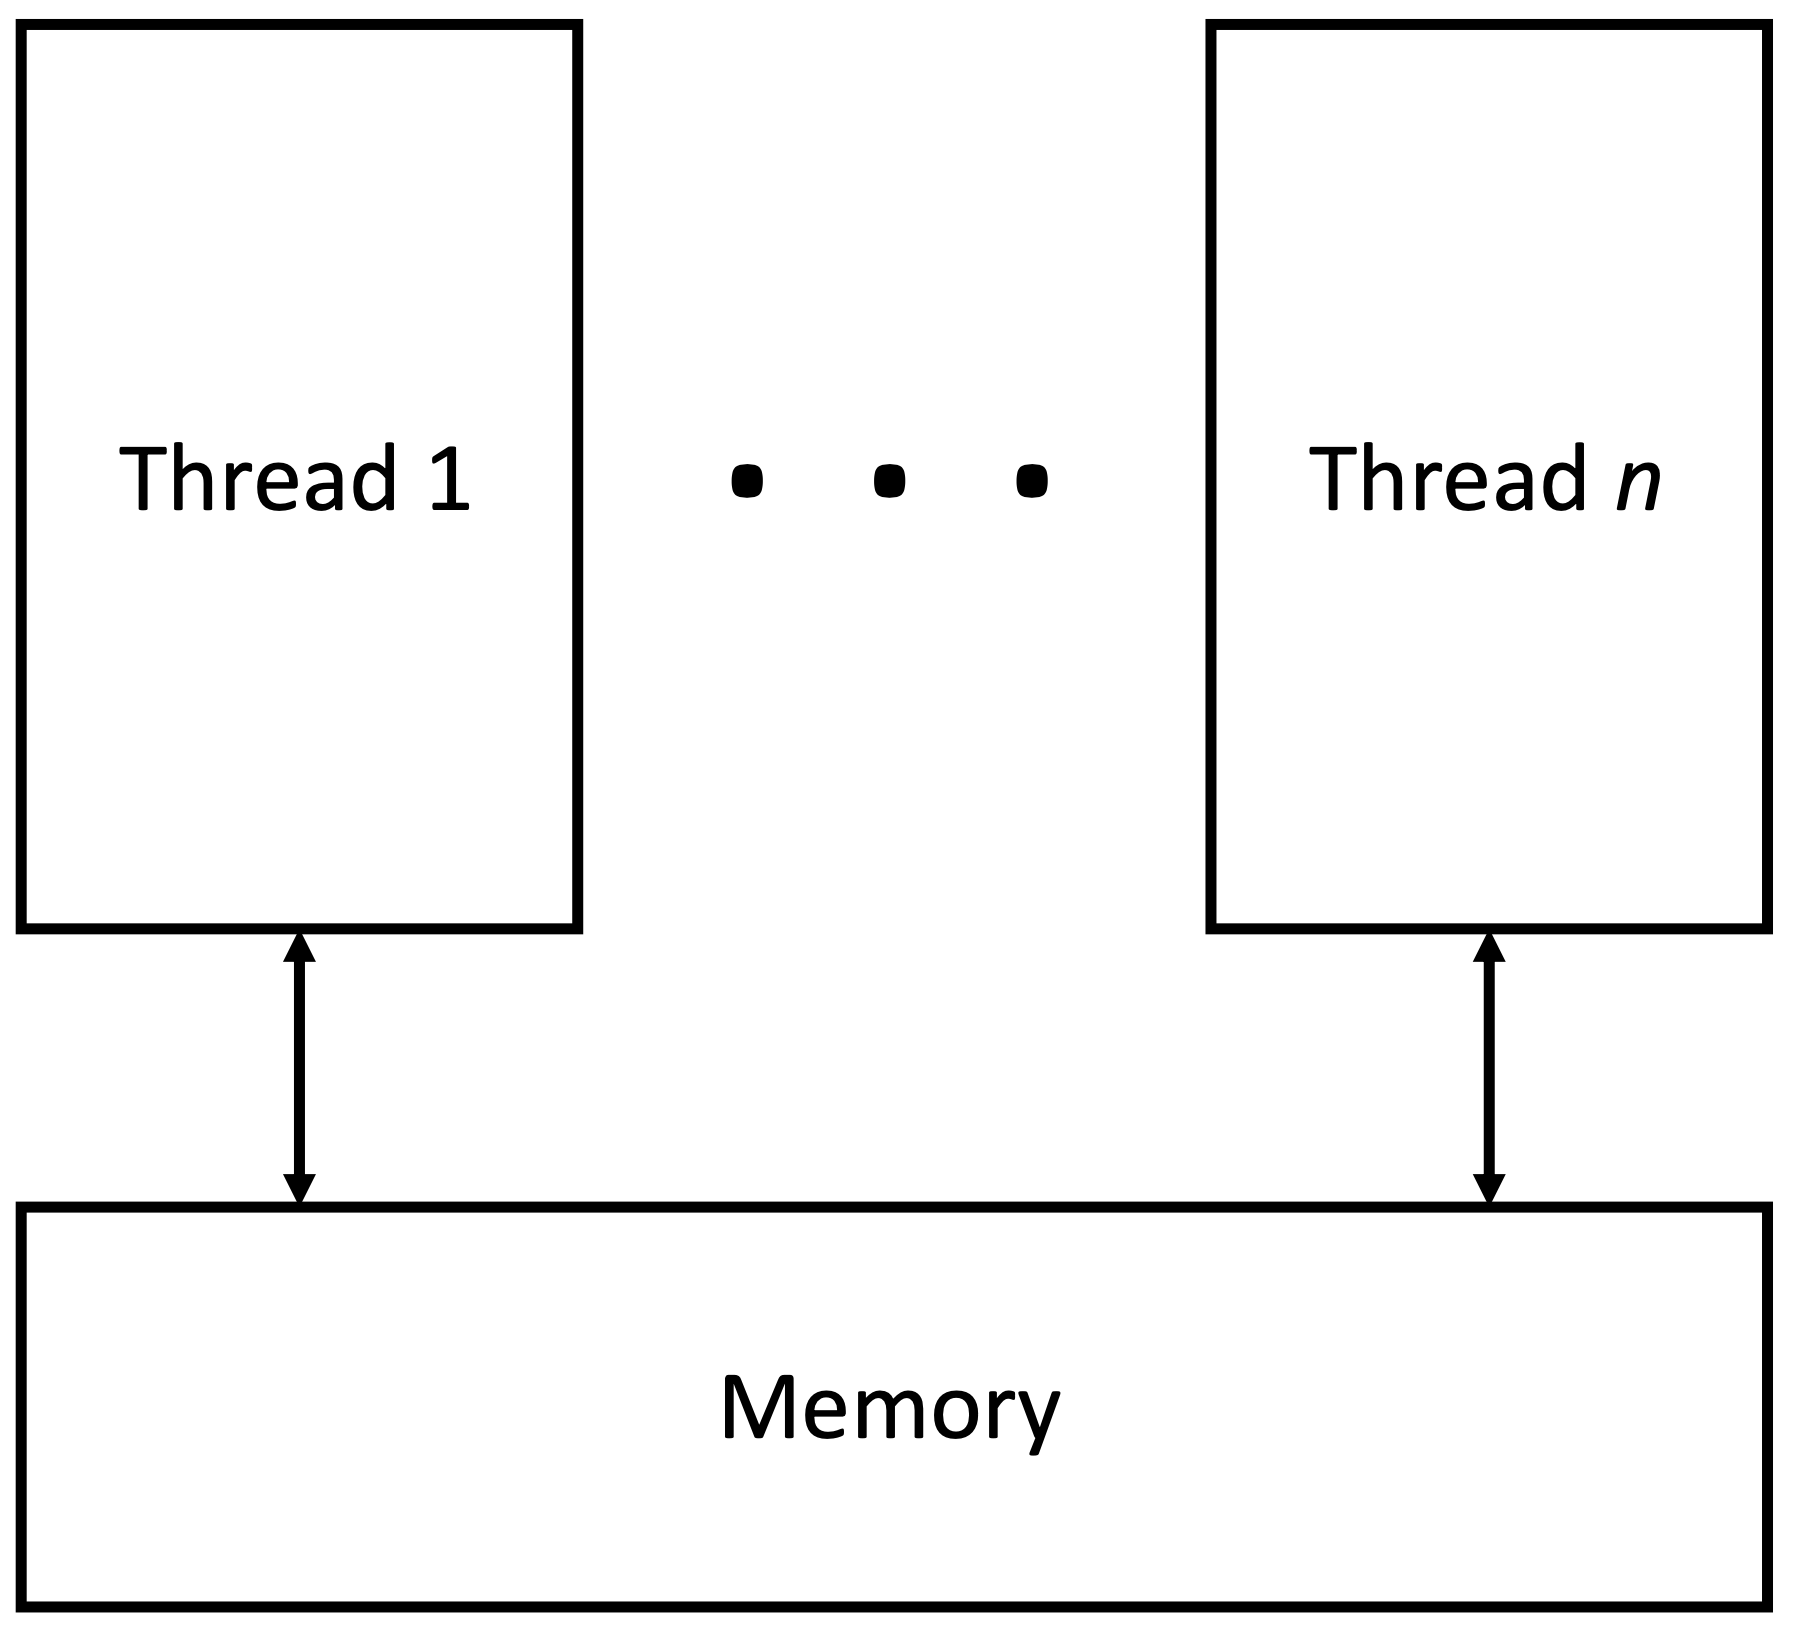
\includegraphics[scale=0.25]{memory.png}
\end{center}
\caption{Memory model}
\label{fig:memory}
\end{figure}

\section{Programs}
\label{sec:programs}
%
Figure \ref{fig:types} summarizes the abstract syntax of \MCMIL.
%
\begin{figure}
\begin{tabular}{llcl}
Values & $v\in\Values$ & = & $\Words$ \\
Addresses & $a\in\Addresses\subseteq\Words$ \\
Registers & $r\in\Regs\subseteq\Words$ \\
Names & $m\in\Names$ \\
Thread identifiers & $\tid\in\Tids$ \\
Types & $\type\in\Types$ & ::= & $\pctype\ \mid\ \regtype\ \mid \ \memtype $ \\
Expressions & $expr\in\Expr$ & ::= & $v\ \mid\ m\ \mid\ \unop(expr)\ \mid\ \binop(expr_1,expr_2)\ \mid\ \cdot$  \\
Messages & $\msgvar\in \Msg$ & ::= & $\tid:m$ \\
Operations & $o\in\Ops$ & ::= & $\expr\  \mid\ \load{\type}{m_a}\ \mid\
\loadsrc{\type}{m_a}{\msgvar}\ \mid \ \store{\type}{m_a}{m_v}$ \\
Microinstructions & $\inst \in \Inst$ & ::= & $\ass{e}{m}{o}$
\end{tabular}
\caption{Types, terms and values}
\label{fig:types}
\end{figure}
%
The \MCMIL\ model inherits much of its syntax and basic ideas from (sequential) \MIL\ \cite{MIL}.

\paragraph{Syntax: Programs, microinstructions, syntactical dependency}
Programs are represented in single static assignment (SSA, \cite{SSA}) form as a sequence of consecutively named microinstructions $\inst$ of the form $\ass{\expr}{m}{o}$ where $m(\inst)=m$ is the name of $\inst$, $c(\inst)=\expr$ is a condition, and $o(\inst) = o$ is an operation, either arithmetic/logic, or load/store. The free names of $\inst$ are the names occurring in $\expr$ and $o$ and the name of $\inst$ is $m$. As in \MIL\ \cite{MIL}, names in \MCMIL\ have a dual role both as microinstruction identifiers and to name the internal resource holding the result of microinstruction evaluation.

The language of microinstructions is straightforward. There are microinstruction for arithmetic and logic operations and loads and stores to/from memory and registers, including the PC which has a particular role in \MIL. Except for loads and stores all microinstructions operate on names rather than immediates or addresses.

The syntactic dependency relation $\depends$ is the transitive closure of the relation $R$ on microinstruction names, such that $m\ R\ m'$ ($m$ depends on $m'$) if $m'$ occurs freely in the instruction bound to (named by) $m$.
For simplicity we assume that all expressions $e$ are strict such that, if $m$ occurs (freely) in $e$ and $m$ is undefined then the value of $e$ is undefined as well. 
Well-formed programs will have the property that $\mbox{$\depends$}\subseteq \mbox{$>$}$, i.e. if $m$ depends on $m'$ then $m'$ is program ordered before $m$.

\paragraph{Threads}
Programs are evaluated per thread. Each thread $\tid\in\Threads$ maintains three components:
\begin{enumerate}
\item
A set $\Dec_\tid\subseteq\Inst$ of decoded microinstructions.
\item
A partial valuation map $\Valuation_\tid$ of names to values.
\item
A set $\Ftch_\tid\subseteq\Names$ of names that have been fetched.
\end{enumerate}
The elaboration of an instruction $\inst$ to the point where all free names
have been assigned a value in $\Valuation_\tid$ enables $\inst$ itself to be evaluated. As result, $\Valuation_{\tid}(m)$ becomes defined as well. Note that
the instruction named by $m$ is \emph{not} the same as the value of $m$.
Rather, $\Valuation_\tid(m)$ is result of evaluating the instruction named by
$m$ in the current state.
Valuations are extended homomorphically to expressions in the usual way. We assume strictness such that if $\Valuation(\expr)\downarrow$ ($\expr$ is defined in $\Valuation$) then $\Valuation(m)\downarrow$ for all $m$ free in $\expr$. 

The set $\Dec_\tid$ represents microinstructions obtained as output of the (macro-) instruction decoding phase, in varying states of elaboration. As in \cite{MIL} we abstract from the details of this encoding.

The set $\Ftch_\tid$ is the set of names of program counter store messages $\store{\pctype}{m_v}$ that have been fetched, causing the ISA instruction encoded as a value $\Valuation_\tid(m_v)$ at location $\Valuation_\tid(m_a)$ to be fetched and decoded.

\paragraph{Messages, Memory, Global States}
%
HERE: attempting to allow ``speculative store forwarding''

Messages $\msgvar\in\Msg$ are ``located'' names: Pairs $\tid:m$ where $m$ names a microinstruction in $\tid$ of the form either a store $\ass{\expr}{m}{\store{\type}{m_a}{m_v}}$, or an annotated load
$\ass{\expr}{m}{\loadsrc{\type}{m_a}{\msgvar}}$. In the latter case, one of two conditions must apply:
%
\begin{enumerate}
\item $\msgvar=\tid:m'$ for some $m'$ such that $m'$ names a store instruction
$\ass{\expr'}{m'}{\store{\type}{m_a'}{m_v'}}$ in $\tid$.
\item $\msgvar = \tid':m'$ for some $\tid'\neq\tid$ and $m'$,
$m'$ names a store instruction
$\ass{\expr'}{m'}{\store{\type}{m_a'}{m_v'}}$ in $\tid'$, and both instructions $m$ and $m'$ are fully defined and enabled.
\end{enumerate}
%
The former case is designed to allow for speculation of the enabling condition $\expr$

if $\msgvar = \tid':m'$ then $m'$ names the store instruction $\store{\type'}{m_a'}{m_v'}$ in $\tid'$ from which the annotated load is assumed to read. Moreover
We call $\msgvar$ the \emph{source} of $m$. This is used to define the happens-before relation below.

The functions $\getName(\msgvar)$, $\getLoc(\msgvar)$, $\getTid(\msgvar)$ are getters used to extract the name, resp. address and tid of message $\msgvar$.

Memory $\mem$ is represented as a set of messages $\tid:m$ where $m$ names a
store microinstruction in $\tid$. This modelling of memory is what ensures multicopy atomicity.

States are pairs $\state = \langle \thrdpool,\mem \rangle\in\States$ of a thread pool $\thrdpool : \Tids\rightarrow \Threads$ and a memory $\mem\subseteq\Msg$.

\section{Semantics: Happens-before}

The tool used in \MCMIL\ to account for instruction scheduling (reordering) is the happens-before relation $\hb$.

The key idea is familar: The happens-before relation must ensure that a
loads read from the most recent completed store that the given thread is able to ``see''. For inter-thread loads completedness is not a problem, since, as we shall see, only completed stores will be visible across threads. For intra-thread reads this is, however, not guaranteed, since, if care is not taken, instruction reordering may cause a store to be completed prior to a PO earlier load whose address or enbledness has not yet been determined. To address this we introduce an additional order, a per-thread ``may-depend'' relation $m\maydepend m'$ ($m$ may depend on $m'$), capturing potential store-to-load dependencies similar to the $\strmay$ function of \cite{MIL}.

\begin{definition}[May-depend]
Let $m$ be a load on address $m_a$, and $m'$ a store $\ass{c'}{m'}{\store{\memtype}{m_a'}{m_v'}}$, both of thread $\tid$. Then $m\maydepend m'$ ($m$ \emph{may depend} on $m'$), if
\begin{enumerate}
\item $m' < m$, and
\item either $\Val{\tid}{c'}$ or $\Val{\tid}{c'}\uparrow$, and
\item either
$\Val{\tid}{m_a}=\Val{\tid}{m_a'}$ or $\Val{\tid}{m_a}\uparrow$ or $\Val{\tid}{m_a'}\uparrow$.
\end{enumerate}
\end{definition}

We can now define the happens-before relation $\hb$:

\begin{definition}[Happens-before]
\label{def:hb}
\mbox{}
\begin{enumerate}
\item Let $A$ be a set of messages and $\state$ a state. Let  $R$ be a relation on $A$ such that $\msg{\tid_1}{m_1}\ R\ \msg{\tid_2}{m_2}$ if either of the following conditions hold:
\begin{enumerate}
\item $\tid_1 = \tid_2$ and $m_2 \depends m_1$.
\item $\tid_1 = \tid_2$, $m_1$ and $m_2$ are both stores, and $m_1$ is maximal such that $m_1 < m_2$. 
\item $m_1$ is a store on $m_a$, $m_2$ is an annotated load on $m_a'$ with source $\msg{\tid_1}{m_1}$, $\Val{\tid_1}{m_a}=\Val{\tid_2}{m_a'}$, and if $\tid_1=\tid_2$ then $m_1$ is maximal under $<$ such that $m_2\maydepend m_1'$ implies $m_1' = m_1$.
\end{enumerate}
\item The state $\state=\langle \thrdpool,\mem\rangle$ is \emph{valid} if the
transitive closure $R^+$ of $R$ is irreflexive.
\item
For valid states the \emph{happens-before} relation $\hb_\state$, or just $\hb$ when the state $\state$ is understood from the context, is the relation $R^+$.
\end{enumerate}
\end{definition}

Notes:
\begin{itemize}
\item Condition \ref{def:hb}.1.a ensures that $\hb$ respects per core syntactic dependencies.
\item Condition \ref{def:hb}.1.b enforces in-order store commits.
\item Condition \ref{def:hb}.1.c is the reads-from relation \cite{readsfrom}.
The maximality condition prevents unelaborated stores from intervening between $m_1$ and $m_2$. \todo[]{Possibly the maximality condition is not needed. It should be ensured by the transition semantics.}
\item Condition \ref{def:hb}.2 ensures that the happens-before relation is causally well-founded (loop-free).
\item The least upper bound under $\hb$ is denoted $\sqcup$.
\end{itemize}
%
Below we show that for reachable states the happens-before relation is irreflexive. 

\subsection{Thread Semantics}
\label{sec:ooo:semantics}
%
We next turn to defining the semantics of microinstructions, in particular the central question ``which value will a given load instruction load?''. To answer this we first define the function $\sources:\Threads \times \Inst\times \Msg\ \mathit{set}\rightarrow \Msg\ \mathit{set}$ that given an unannotated, i.e. not yet evaluated, load microinstruction $\inst = \ass{c}{m}{\load{\type}{m_a}}$ executing at thread $\tid$ and a set $A$ of messages representing the current shared set of messages returns the set of store microinstructions that $\inst$ may read from:
%
\begin{eqnarray*}
\lefteqn{\sources(\tid,m,A)} \\
 & = & 
\{\msgvar' \mid
\msgvar'\mbox{ is maximal under }\hb, \Val{\tid}{m_a} = \getLoc(\msgvar'),\mbox{ and if }\tid = \getTid(\msgvar') \\
 & & \mbox{ then }\getName(\msgvar')\mbox{ is maximal under $<$ s.t. }
m \maydepend m''\mbox{ implies }m''=\getName(\msgvar')
\}
\end{eqnarray*}
%
Relating to the \emph{str-may} and \emph{str-act} sets of \cite{inspectre}, let
$\ass{c}{m}{\load{\type}{m_a}}$ be a given load instruction. Then:
%
\begin{eqnarray*}
\lefteqn{\strmay(\tid,m,A)} \\
 & = & \{\ass{c'}{m'}{\store{\type}{m_a'}{m_v'}}\mid
m' < m \wedge (\Val{\tid}{c'} \vee \Val{\tid}{c'}\uparrow) \wedge \mbox{} \\
 &   & (\Val{\tid}{m_a}=\Val{\tid}{m_a'} \vee \Val{\tid}{m_a}\uparrow \vee
\Val{\tid}{m_a'}\uparrow) \\
\lefteqn{\stract(\tid,m,A)} \\
 & = & \{\ass{c'}{m'}{\store{\type}{m_a'}{m_v'}} \in \strmay(\tid,m,A)\mid\mbox{} \\
 &   & \neg\exists\ass{c''}{m''}{\store{\type}{m_a''}{m_v''}}\in\strmay(\tid,m,A).m''>m'\wedge \Val{\tid}{c''}\wedge \Val{\tid}{m_a''} \in\{\Val{\tid}{m_a},\Val{\tid}{m_a'}\}
\end{eqnarray*}
%
We obtain:
%
\begin{proposition}
Let instructions $\inst=\ass{c}{m}{\load{\type}{m_a}}$,
$\inst' = \ass{c'}{m'}{\store{\type}{m_a'}{m_v'}}$ be given.
\begin{enumerate}
\item $\inst'\in \strmay(\tid,m,A)$ iff
$m\maydepend m'$.
\item $\inst'\in\stract(\tid,m,A)$ is fully defined and enabled iff
$\msgvar' = \tid:m'\in\Msg\cap\sources(\tid,m,A)$. 
\end{enumerate}
\end{proposition}
\begin{proof}
1. Trivial.

\noindent 2. If: Suppose $\msgvar' = \tid:m'\in\Msg\cap\sources(\tid,m,A)$.
Since $\tid:m'\in\Msg$, $\ass{c'}{m'}{\store{\type}{m_a'}{m_v'}}\in\strmay(\tid,m,A)$ is enabled and fully
defined. Also, $\Val{\tid}{m_a}=\Val{\tid}{m_a'}$. Maximality ensures that no $m''$ exists PO-after
$m'$ and PO-prior to $m$, which concludes.
Only-if: Suppose $\msgvar'\in\stract(\tid,m,A)$. Then $\msgvar'\in\Msg$.
STOP


\end{proof}


BREAK



To define the transition relation we first assign a return value to instructions using the operation $[\msg{\tid}{\inst}](\state)$ as follows.
Let $\state=(\thrdpool,\mem)$ and $\thrdpool(\tid)=(\Dec,\Valuation,\Ftch)$:
%
\begin{itemize}
\item $[\msg{\tid}{\ass{c}{m}{e}}](\state) =
\left \{
  \begin{array}{ll}
     \Val{\tid}{e} & \mbox{if }\Val{\tid}{e}\downarrow\mbox{ and }\models\Val{\tid}{c} \\
     \perp & \mbox{otherwise}
   \end{array}
 \right.
$
\item $[\msg{\tid}{\ass{c}{m}{\store{\type}{m_a}{m_v}}}](\state) = 
    \left \{
      \begin{array}{ll}
        \Val{\tid}{m_v} &  \mbox{if } \Val{\tid}{m_v}\downarrow, \mbox{ and } \Val{\tid}{m_a}\downarrow, \mbox{ and }
                     \models\Val{\tid}{c} \\
        \perp & \mbox{otherwise}
      \end{array}
    \right .
$
\end{itemize}
%
For loads we first define the helper function $\src{\cdot}$ determining load sources:
%
\begin{itemize}
\item $
\src{\msg{\tid}{\ass{c}{m}{\load{\type}{m_a}}}} =
    \left \{
      \begin{array}{ll}
        \msgvar & \msgvar = \msg{\tid'}{\ass{c'}{m'}{\store{\type}{m_a'}{m_v'}}}
                  \in\Dec_{\tid}\cup\mem \\
                & \mbox{is maximal under }\hb\mbox{ s.t. } \\
                & \msgvar\mbox{ is enabled, }\Val{\tid}{m_a}=\Val{\tid'}{m_a'} \\
                & \hb\mbox{ and, if }\tid'=\tid \mbox{ then there} \\
                & \mbox{does not exist }\msg{\tid}{m''}\in\Dec_{\tid} \mbox{ for which } \\
                & m'\maydepend m''\maydepend m \\
        \perp & \mbox{otherwise}
      \end{array}
    \right.
    $
\item $
[\msg{\tid}{\ass{c}{m}{\load{\type}{m_a}}}](\state)  = 
    \left \{
      \begin{array}{ll}
        \Val{\tid'}{m_v'} & \mbox{if }\models\Val{\tid}{c}\mbox{ and } \\
                   & \src{\msg{\tid}{\ass{c}{m}{\load{\type}{m_a}}}} = \\
                   &  \msg{\tid'}{\ass{c'}{m'}{\store{\type}{m_a'}{m_v'}}} \\
        \perp & \mbox{otherwise}
      \end{array}
    \right.
    $
\end{itemize}

We explain the intuition behind the above definition. First, assume that the load $\msg{\tid}{m}$ reads from the store $\msg{\tid'}{m'}$ and $\tid\neq \tid'$,
i.e. such that $\Dec_{\tid}{m_a} = \Dec_{\tid'}{m_a'}$. Then $\msgvar$ is maximal under $\hb$ with this property, since otherwise $\tid$ reads from the distant past. Conversely, if $m'$ \emph{is} maximal and writes to $\Dec_{\tid'}{m_a'}=\Dec_{\tid}{m_a}$ then there is a schedule that causes $m$ to read from $m'$.

If on the other hand $m$ reads from $m'$ and $\tid = \tid'$. Then $m'$ must be
defined and enabled, and $\Dec_{\tid}(m_a) = \Dec_{\tid'}(m_a')$. Also $\msgvar$ must be the largest such store under $\hb$. Also no store $m''$ between $m'$ and $m$ should exist, since that would have caused $m$ to read from the distant past. Conversely, if $m'$ as above exists with $\Dec_{\tid}{m_a}=\Dec_{\tid}{m_a'}$,
$\msgvar$ maximal under $\hb$, and no $m''$ as above in existence. Then it is possible by suitable scheduling for $m$ to read from $m'$.

Need to prove some propositions about this.

It should be possible to show equivalence with a definition in the style of $\strmay$/$\stract$. TODO.

Next the transition rules consisting of five execution steps and two ``non-execution'' steps, for commit and fetch, respectively. Later, we introduce additional non-execution steps for concurrency control.
We use $\tid:m\parallel P$ or $\tid:(\Dec,\Valuation,\Ftch)\parallel P$ to denote the
threadpool $P[\tid\mapsto m]$, alt. $P[\tid\mapsto(\Dec,\Valuation,\Ftch)]$. Forthe transition rules to follow let $\state=(\tid:(\Dec, \Valuation, \Ftch)\parallel\thrdpool,\mem)$:

  \[
    \begin{array}{cc}
(\xp)
&
\begin{array}{c}
  \inst = \ass{c}{m}{e}  \in \Dec \qquad \Val{\tid}{m}\uparrow \qquad
  [\msg{\tid}{\inst}](\state) = v
\\ \hline
\state \rightarrow (\tid:(\Dec,
\subst{\Valuation_{\tid}}{m}{v}, \Ftch)\parallel\thrdpool,\mem)
\end{array}\\
\end{array}
\]

\[
\begin{array}{cc}
(\sto)
&
\begin{array}{c}
  \inst = \ass{c}{m}{\store{\type}{m_a}{m_v}}\in\Dec \qquad \Val{\tid}{m}\uparrow \qquad
  [\msg{\tid}{\inst}](\state) = v
\\ \hline
\state \rightarrow (\tid:(\Dec,
\subst{\Valuation_{\tid}}{m}{v}, \Ftch)\parallel\thrdpool,\mem)
\end{array}\\
\end{array}
\]

\[
    \begin{array}{cc}
(\ldregpc)
&
\begin{array}{c}
  \inst = \ass{c}{m}{\load{\type}{m_a}}  \in \Dec \qquad \Val{\tid}{m}\uparrow \qquad [\msg{\tid}{\inst}](\state) = v \qquad \type\neq\memtype
\\ \hline
\state \rightarrow (\tid:(\Dec,
\subst{\Valuation_{\tid}}{m}{v}, \Ftch)\parallel\thrdpool,\mem)
\end{array}\\
\end{array}
\]

\[
    \begin{array}{cc}
(\ldthrd)
&
\begin{array}{c}
  \inst = \ass{c}{m}{\load{\memtype}{m_a}}  \in \Dec \qquad \Val{\tid}{m}\uparrow \qquad [\msg{\tid}{\inst}](\state) = v
  \qquad \src{\msg{\tid}{\inst}} \in\Dec
\\ \hline
\state \rightarrow (\tid:(\Dec,
\subst{\Valuation_{\tid}}{m}{v}, \Ftch)\parallel\thrdpool,\mem)
\end{array}\\
\end{array}
\]

Note: The source thread $\tid'$ is forced to be $\tid$ since $\src{\msg{\tid}{\inst}}\in\Dec$.

\[
    \begin{array}{cc}
(\ldmem)
&
\begin{array}{c}
  \inst = \ass{c}{m}{\load{\memtype}{m_a}}  \in \Dec \qquad \Val{\tid}{m}\uparrow \qquad [\msg{\tid}{\inst}](\state) = v
  \qquad  \src{\msg{\tid}{\inst}} = \msg{\tid'}{\inst'}\in\mem
\\ \hline
\state \rightarrow (\tid:(\Dec\setminus\{m\},
\subst{\Valuation_{\tid}}{m}{v}, \Ftch)\parallel\thrdpool,\mem\cup\{\msg{\tid}{\ass{c}{m}{\loadsrc{\type}{m_a}{\src{\msg{\tid}{\inst}}}}}\})
\end{array}\\
\end{array}
\]

Note: The effect of this rule is to propagate memory loads to memory while adding the source annotation.

\[
    \begin{array}{cc}
(\cmt)
&
\begin{array}{c}
  \inst = \ass{c}{m}{\store{\memtype}{m_a}{m_v}} \in \Dec \qquad
  \Val{\tid}{m}\downarrow \qquad
  \msg{\tid}{\inst} \notin \mem \qquad 
  \{\msg{\tid'}{\inst'}\mid \msg{\tid'}{\inst'}\hb \msg{\tid}{\inst}\} \subseteq \mem \\ \hline
\state\rightarrow (\tid:(\Dec,\Valuation_{\tid},\Ftch)\parallel\thrdpool,\mem\cup
\{\msg{\tid}{\inst}\})
\end{array}
\end{array}
\]
%
Prove that $\{m'\mid m\maydepend m'\}\subseteq \mem$ if $m\in\mem$

\[
    \begin{array}{cc}
(\ftc)
&
  \begin{array}{c} 
    \inst = \ass{c}{m}{\store{\pctype}{}{m_v}} \in \Dec \qquad
    \Val{\tid}{m}=v \qquad
    m \notin \Ftch \qquad
    \{m'\mid m'< m\} \subseteq \Ftch \\ \hline
    \state\rightarrow (\tid:(\Dec\cup\translate(v, max(\Dec)),\Valuation_{\tid},\Ftch\cup\{\msg{\tid}{\inst}\})\parallel\thrdpool,\mem)
  \end{array}
      \end{array}
\]
%
Instructions are fetched in program order.
%
\paragraph{Initial states}
An initial state is any state $\state_0 = \langle \thrdpool,\mem\rangle$ such that:
\begin{itemize}
\item $\Dec_\tid=\{\ass{\top}{m_0}{\store{\pctype}{}{v}} \}$ where $v$ encodes the first instruction to be executed by thread $\tid$, $\Valuation_\tid = \bot$, and $\Ftch = \emptyset$.
\item $\mem = \{ \ass{\top}{0}{\store{\memtype}{a}{0}} \mid a\ \mathit{address} \}$.
\end{itemize}
%
Note that each transition directly affects exactly one thread.
We refer to a transition justified by one of {\sc Exp}, {\sc Sto}, {\sc LdRPC}, {\sc LdT}, or {\sc LdM} as an \emph{execution step}.
Say that a transition $\state\rightarrow\state'$ \emph{introduces the message} $\msg{\tid}{m}$, if the transition is by thread $\tid$, and $m$ is the bound name of the executed instruction. Note that only execution steps introduce messages and introduced messages are unique.

\section{Preservation of Validity}

We prove that validity is preserved under transition in order to justify our definition of happens-before. For this purpose we from now on restrict attention to reachable states and assume a well-formedness condition that is preserved under transitions. This allows to prove the impossibility of loops in the happens-before relation for states, since an unreachable state violating the condition is trivial to construct. 

By the discussion above we immediately get:

\begin{proposition}
\label{prop:introducing}
If $\state=\langle\thrdpool,\mem\rangle\rightarrow\state'=\langle\thrdpool',\mem'\rangle$ then either $\mem'=\mem$ or $\mem'= \mem\cup \{\msg{\tid}{m}\}$ where
$m$ is the name introduced by the transition $\state\rightarrow\state'$ and $\mem'=\mem$. \hfill $\Box$
\end{proposition}

\begin{proposition}
\label{prop:depends}
Suppose that $\state=\langle\thrdpool,\mem\rangle\rightarrow\state'=\langle\thrdpool',\mem'\rangle$ introduces the message $\msg{\tid}{m_2}$. Then
$m_1\not\depends m_2$ for any message  $\msg{\tid}{m_1}\in\mem$.
\end{proposition}
\begin{proof}
Pick $\msg{\tid}{m_1}\in\mem$. If $m_1\depends m_2$ the instruction
binding $m_1$ has a free name. Then $m_1$ is not in the initial memory, and it is not added in an execution step. The conclusion follows.
\end{proof}

\begin{theorem}
Suppose $\state\rightarrow \state'$ and $\state$ is valid. Then $\state'$ is valid.
\end{theorem}
\begin{proof}
If state validity is not invariant then we find a transition
$\state\rightarrow \state'$ for which $\hb_{\state}$ is irreflexive and
$\hb_{\state'}$ is reflexive. Let $m$ be the name introduced by the transition
$\state\rightarrow \state'$. Such a name must exist since otherwise
$\hb_\state=\hb_{\state'}$. Then we find a maximal $\hb_{\state'}$-chain
\[
\msg{\tid}{m} = \msg{\tid_0}{m_0}\hb_{\state'}\cdots \hb_{\state'}\msg{\tid_n}{m_n} = \msg{\tid}{m}
\]
with one of the conditions \ref{def:hb}.1.a-c holding at each step. Moreover, we can arrange the chain such that to each message $\msg{\tid_i}{m_i}$, $0 < i \leq m$, is associated a transition $\state_{i-1}\rightarrow \state_i$ introducing $m_i$, and in this way construct a derivation $\state_0\rightarrow^+
\state_1 =\rightarrow^+ \cdots \rightarrow^+ \state_{n-1} \rightarrow^+ \state_n$
such that $\state_{n-1} = \state$ and $\state_n = \state'$. (The unlisted intermediate states in this derivation are states elaborated due to commit or fetch transitions that do not introduce a name).

Since each instance of rules \ref{def:hb}.a and \ref{def:hb}.b stricly decreases $<$, which is well-founded, at least one of the transitions $\state_{i-1}\rightarrow \state_i$ must be an instance of \ref{def.hb}.c. It follows there must exist a subsequence $\state_0'\rightarrow^+
\state_1' =\rightarrow^+ \cdots \rightarrow^+ \state_{m-1}' \rightarrow^+ \state_m'$ such that each transition $\state_{j-1}'\rightarrow^+ \state_{j}$ consists of a number of instances commit or fetch transitions, or there are  

\end{proof}
%
HER

%
\section{Barriers and Concurrency Control}
%
\todo[inline]{Needs updating}
We next turn to barriers and concurrency control instructions.
At microinstruction level these functionalities are represented separately from their associate memory operations. 
We thus introduce a collection of new operations, acquire, release, exclusive access (lr/sc), fences, and begin/end of atomic regions:
\[
\begin{array}{l}
\btype ::= R\ \mid\ W\ \mid\ RW \\
o ::= \ldots \mid\ \acq{\btype}\ \mid\ \rel{\btype}\ \mid\ \loadr{t}\ \mid\ \storec{t_a}{t_v}\mid\ \fence{\btype}
\end{array}
\]
In order to account for this extension in a modular way we introduce a
new transition arrow  $\rightarrowtail$ defined using $\rightarrow$.

\paragraph{Acquire}
%
The key idea of an acquire barrier instruction $\ass{c}{t}{\acq{\btype}}$ is that microinstructions of type $\btype$ that appear PO-after $t$ must not be executed prior to the barrier. We implement this by requiring
\begin{enumerate}
\item The acquire barrier (as for other barriers below) to be executed in program order.
\item Any microinstructions of type $\btype$ to be executed only when all PO-prior acquire barriers have been committed.
\end{enumerate}
%
At operation level an acquire instruction return the unit value $\unit$.
\[
\den{\ass{c}{t}{\acq{\btype}}} = \unit
\]
At transition level acquire instructions require a transition rule on their own that just expresses and records that the acquire is evaluated and committed in program order:
%
\[
\begin{array}{cc}
(\mbox{\sc{Acq}})
&
\begin{array}{c}
  t\notin\Commits \qquad
  \den{c}{\storage} \qquad
  t<t' \wedge t':\btype\wedge\tid(t) = \tid(t')\Rightarrow t'\notin\Commits \\ \hline
(\ass{c}{t}{\acq{\btype}},\Inst, \storage, \Commits, \Decodes) \rightarrowtail (\Inst,\storage, \Commits\cup\{t\}, \Decodes)
\end{array}
\end{array}
\]
%
In formulating this rule we use $x,X$ as a shorthand for the set $\{x\}\cup X$ where $x\notin X$. (This can be used to simplify other rules as well).

\paragraph{Release}
Releases require that any PO-prior microinstruction of an appropriate type have been committed. 
%
Again we let:
%
\[
\den{\ass{c}{t}{\rel{\btype}}}=\unit
\]
Releases are executed in program order:
%
\[
\begin{array}{cc}
\mbox{\sc{Rel}} &
\begin{array}{c}
t\notin\Commits \qquad
\den{c}{\storage} \qquad
t'<t \wedge t':\btype \wedge\tid(t) = \tid(t') \Rightarrow t'\in\Commits \\ \hline
(\ass{c}{t}{\rel{\btype}},\Inst, \storage, \Commits, \Decodes)\rightarrowtail
(\Inst,\storage,\Commits\cup\{t\},\Decodes)
\end{array}
\end{array}
\]
%
\paragraph{Exclusive access}
To model exclusive access ($\loadr{}{}$/$\storec{}{}$) we add an exclusive bank to the state. The exclusive bank $\exclusives$ is a partial map taking memory location $\loc$ to thread id's $\tid$ holding the reservation on $\loc$, when applicable. Thus the state will here have the shape $(\Inst,\storage,\Commits,\Decodes,\exclusives)$. This change is a bit more intrusive than previously since it affects also regular stores. 

At the single operation level a load-reserved acts as a regular load:
\[
\den{\ass{c}{t}{\loadr{t_a}}}\newstate = \den{\ass{c}{t}{\load{\restypemem}{t_a}}}\newstate
\]
and a store conditional as a regular store:
\[
\den{\ass{c}{t}{\storec{t_a}{t_v}}}\newstate = \den{\ass{c}{t}{\store{\restypemem}{t_a}{t_v}}}\newstate
\]

For the transitions:

\noindent \textbf{Load-reserved} 
  \[
    \begin{array}{cc}
(\mbox{\sc LR})
&
\begin{array}{c}
  \inst =  \ass{c}{t}{\loadr{t_a}{t_v}}  \in \Inst \qquad \fundefined{\storage}{t} \qquad
\den{c}{\storage} \qquad \den{\inst}\newstate = v
\\ \hline
\newstate = (\Inst, \storage, \Commits, \Decodes,\exclusives) \rightarrow (\Inst,\subst{\storage}{t}{v}, \Commits, \Decodes,\exclusives[\den{t_a}\mapsto\tid(t)]
\end{array}\\
\end{array}
\]
%
The only difference between a plain load and the load reserved is the effect on the exclusive bank. The load reserved will scratch any reservation currently in effect and grab the reservation for the current thread. The plain load, shown below, will have either no effect on the exclusive bank (and so this rule is left out), or alternatively a load reserved will cause the reservation flag to be lifted, as shown below.

\noindent \textbf{Load v2} 
  \[
    \begin{array}{cc}
(\mbox{\sc Load})
&
\begin{array}{c}
  \inst =  \ass{c}{t}{\loadr{t_a}{t_v}}  \in \Inst \qquad \fundefined{\storage}{t} \qquad
\den{c}{\storage} \qquad \den{\inst}\newstate = v
\\ \hline
\newstate = (\Inst, \storage, \Commits, \Decodes,\exclusives) \rightarrow (\Inst,\subst{\storage}{t}{v}, \Commits, \Decodes,\exclusives[\den{t_a}\mapsto\bot]
\end{array}\\
\end{array}
\]
%
\noindent \textbf{Store Conditional} 
  \[
    \begin{array}{cc}
(\mbox{\sc SC1})
&
\begin{array}{c}
  \inst =  \ass{c}{t}{\storec{t_a}{t_v}}  \in \Inst \qquad \fundefined{\storage}{t} \qquad
\den{c}{\storage} \qquad \den{\inst}\newstate = v \qquad
\exclusives(\den{t_a}) = \tid(t)
\\ \hline
\newstate = (\Inst, \storage, \Commits, \Decodes,\exclusives) \rightarrow (\Inst,\subst{\storage}{t}{v}, \Commits, \Decodes,\exclusives[\den{t_a}\mapsto\bot]
\end{array}\\
\end{array}
\]
%
The effect of a store conditional, assuming the executing thread has the reservation, is to quash the reservation.
%
  \[
    \begin{array}{cc}
(\mbox{\sc SC2})
&
\begin{array}{c}
  \inst =  \ass{c}{t}{\storec{t_a}{t_v}}  \in \Inst \qquad \fundefined{\storage}{t} \qquad
\den{c}{\storage} \qquad \den{\inst}\newstate = v \qquad
\exclusives(\den{t_a}) \neq \tid(t)
\\ \hline
\newstate = (\Inst, \storage, \Commits, \Decodes,\exclusives) \rightarrow (\Inst,\storage, \Commits, \Decodes,\exclusives[\den{t_a}\mapsto\bot]
\end{array}\\
\end{array}
\]
%
This case applies when either no reservation is taken on $\den{t_a}$ or a reservation is taken, but by another thread.
Probably this is wrong since the storage needs to record that the store conditional was executed but unsuccessful and not leave it undefined.
%
\noindent \textbf{Store} 
  \[
    \begin{array}{cc}
(\mbox{\sc Store})
&
\begin{array}{c}
  \inst =  \ass{c}{t}{\store{t_a}{t_v}}  \in \Inst \qquad \fundefined{\storage}{t} \qquad
\den{c}{\storage} \qquad \den{\inst}\newstate = v
\\ \hline
\newstate = (\Inst, \storage, \Commits, \Decodes,\exclusives) \rightarrow (\Inst,\subst{\storage}{t}{v}, \Commits, \Decodes,\exclusives[\den{t_a}\mapsto\bot]
\end{array}\\
\end{array}
\]
%
The effect of a store is always to quash the reservation, if any.
